\begin{figure}
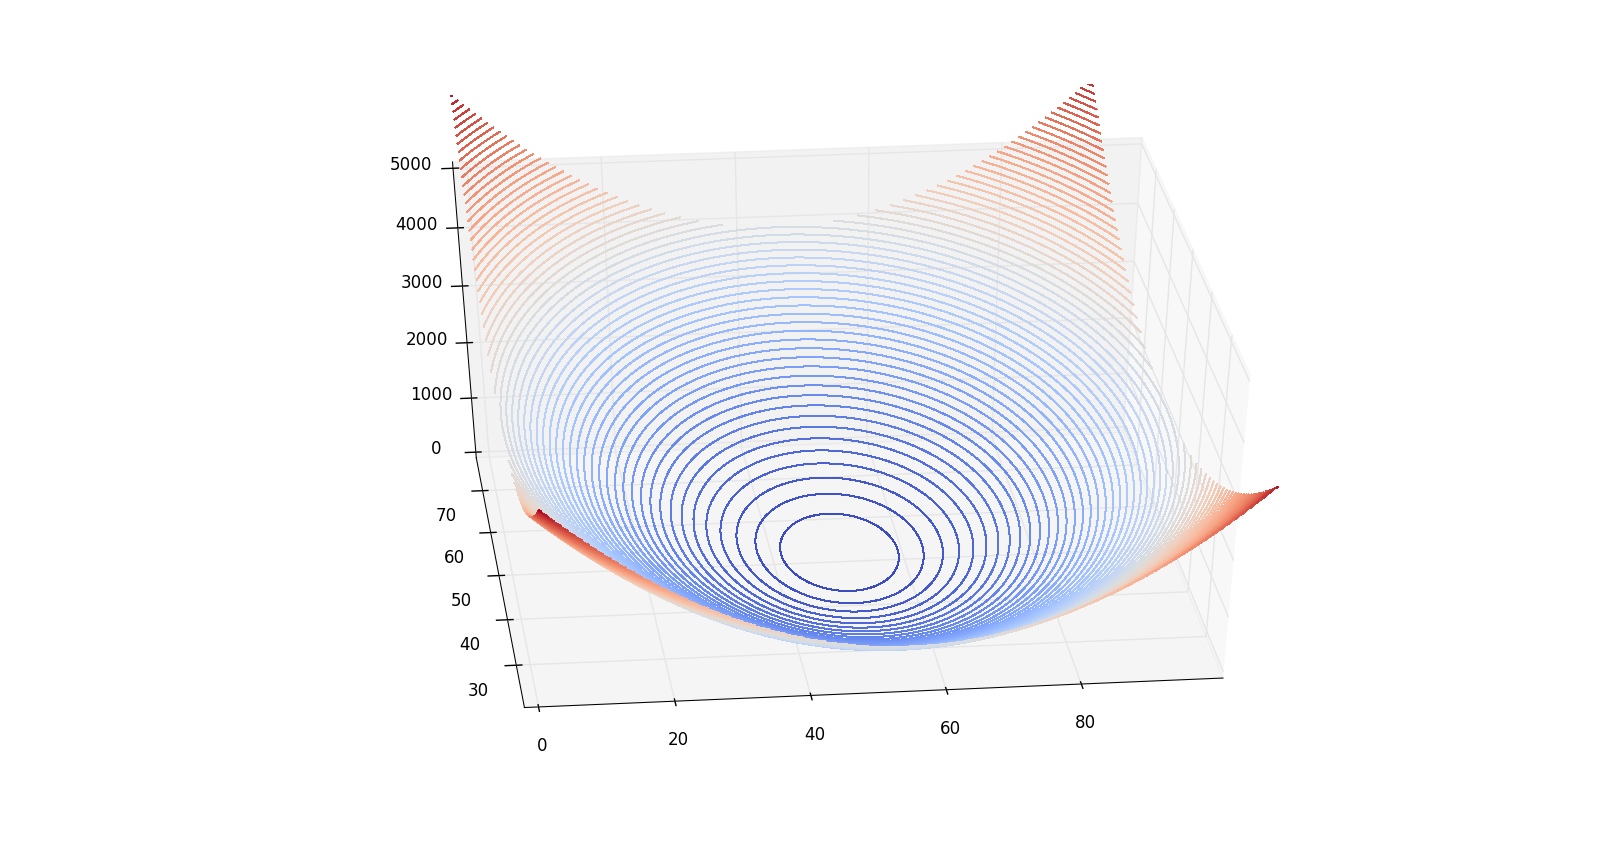
\includegraphics[height=.3\vsize]{fig/arriv1.png}
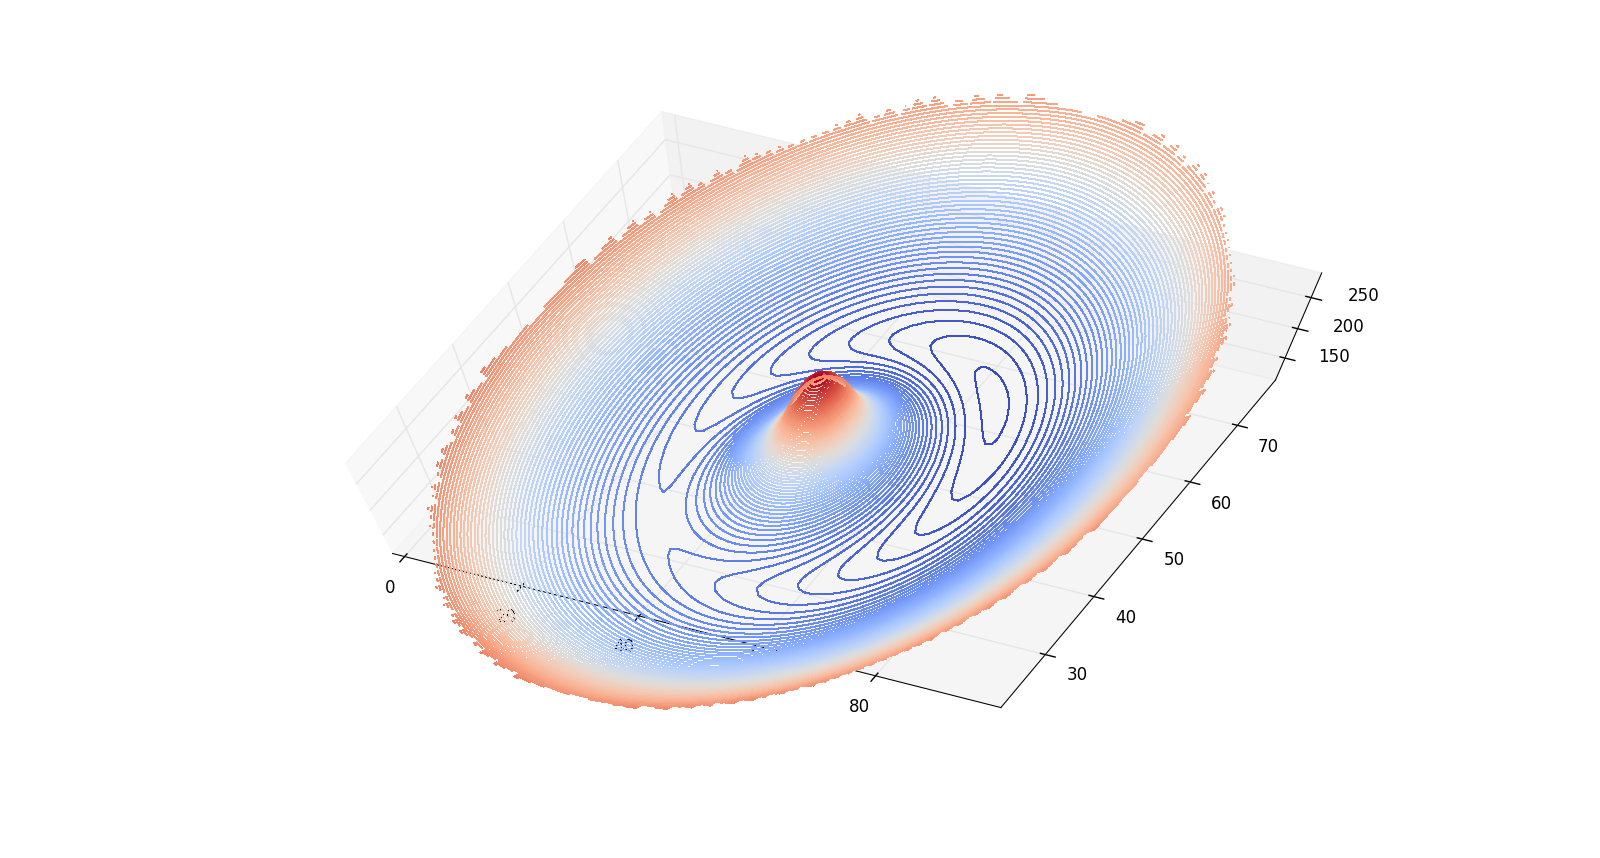
\includegraphics[height=.3\vsize]{fig/arriv2.png}
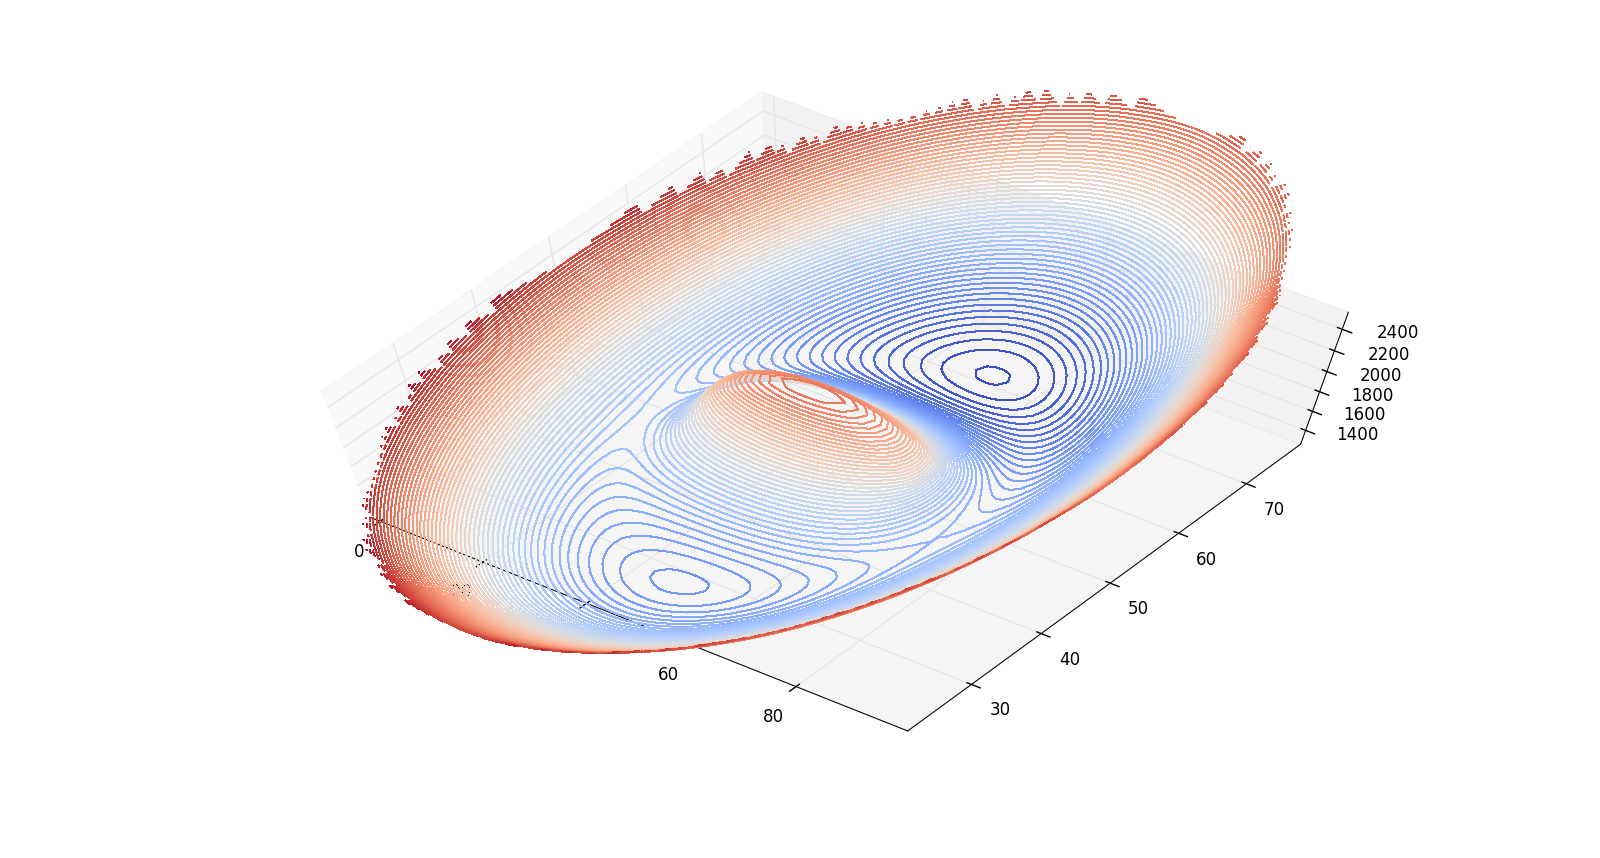
\includegraphics[height=.3\vsize]{fig/arriv3.png}
\caption{Arrival-time surfaces\label{fig:arriv}}
\end{figure}

\section{Fermat's Principle} \label{sec:Fermat}

There are several ways to understand the formation of arcs and
multiple images in gravitational lensing.  We will follow an approach
originally introduced by \cite{1986ApJ...310..568B}, based on Fermat's
principle.

\begin{equation}
\hbox{arrival time} = A_{\rm geom} - A_{\rm grav}
\end{equation}
By convention, $A_{\rm grav}$ is defined in such a way that it is
negative, hence the minus sign.

Although $A_{\rm geom}$ and $A_{\rm grav}$ are times, we are going to
write them as if they are areas.  In other words, we will suppress a
constant factor in the $A$.  That factor is basically the lens
distance times the speed of light, but the precise expression is given
in the Appendix.

Introduce the Laplacian $\nabla^2 f(x,y)$ is
\begin{equation}
 \frac{ f(x+\Delta x, y) + f(x-\Delta x, y) +
        f(x, y+\Delta y) + f(x, y-\Delta y) - 4 f(x,y) }
      {\Delta x \; \Delta y}
\end{equation}
in the limit of $\Delta x,\Delta y$ small.

Let $x,y$ be coordinates on the lens, transverse to the line of sight.
Let there be a point source behind $x=0,y=0$.  Then
\begin{equation}
A_{\rm geom}(x,y) = \half(x^2 + y^2)
\end{equation}
\begin{equation}
\nabla^2 A_{\rm grav}(x,y) = 2\kappa(x,y)
\end{equation}
Here $\kappa$ is a dimensionless quantity with two distinct physical
interpretations.  On the one hand, it is the sky projected density ---
in special units, to make it dimensionless.  On the other hand,
$\kappa$ is the {\em convergence\/} of a bundle of rays.
